% README 训练/评测管线图（与论文插图同一套 TikZ 风格；信息落在方框内 + 底部一行契约）
% 编译：见同目录 build_diagrams.sh
\documentclass[border=8pt]{standalone}
\usepackage{fontspec}
\setmainfont{Liberation Sans}
\usepackage{tikz}
\usetikzlibrary{arrows.meta, positioning, fit, backgrounds, calc}

\definecolor{cblue}{RGB}{31, 78, 121}
\definecolor{camber}{RGB}{197, 90, 17}
\definecolor{cgreen}{RGB}{46, 125, 50}
\definecolor{clink}{RGB}{90, 90, 90}

\tikzset{
  box/.style={draw=clink, line width=1.1pt, rounded corners=3pt, align=center,
              inner sep=5pt, font=\fontsize{13}{15}\selectfont},
  arr/.style={-{Stealth[length=5pt]}, line width=1.4pt, draw=clink},
  lab/.style={font=\fontsize{12.5}{14}\selectfont, color=clink, align=center},
  grp/.style={draw=clink!55, dashed, rounded corners=4pt, inner sep=7pt},
}

\begin{document}
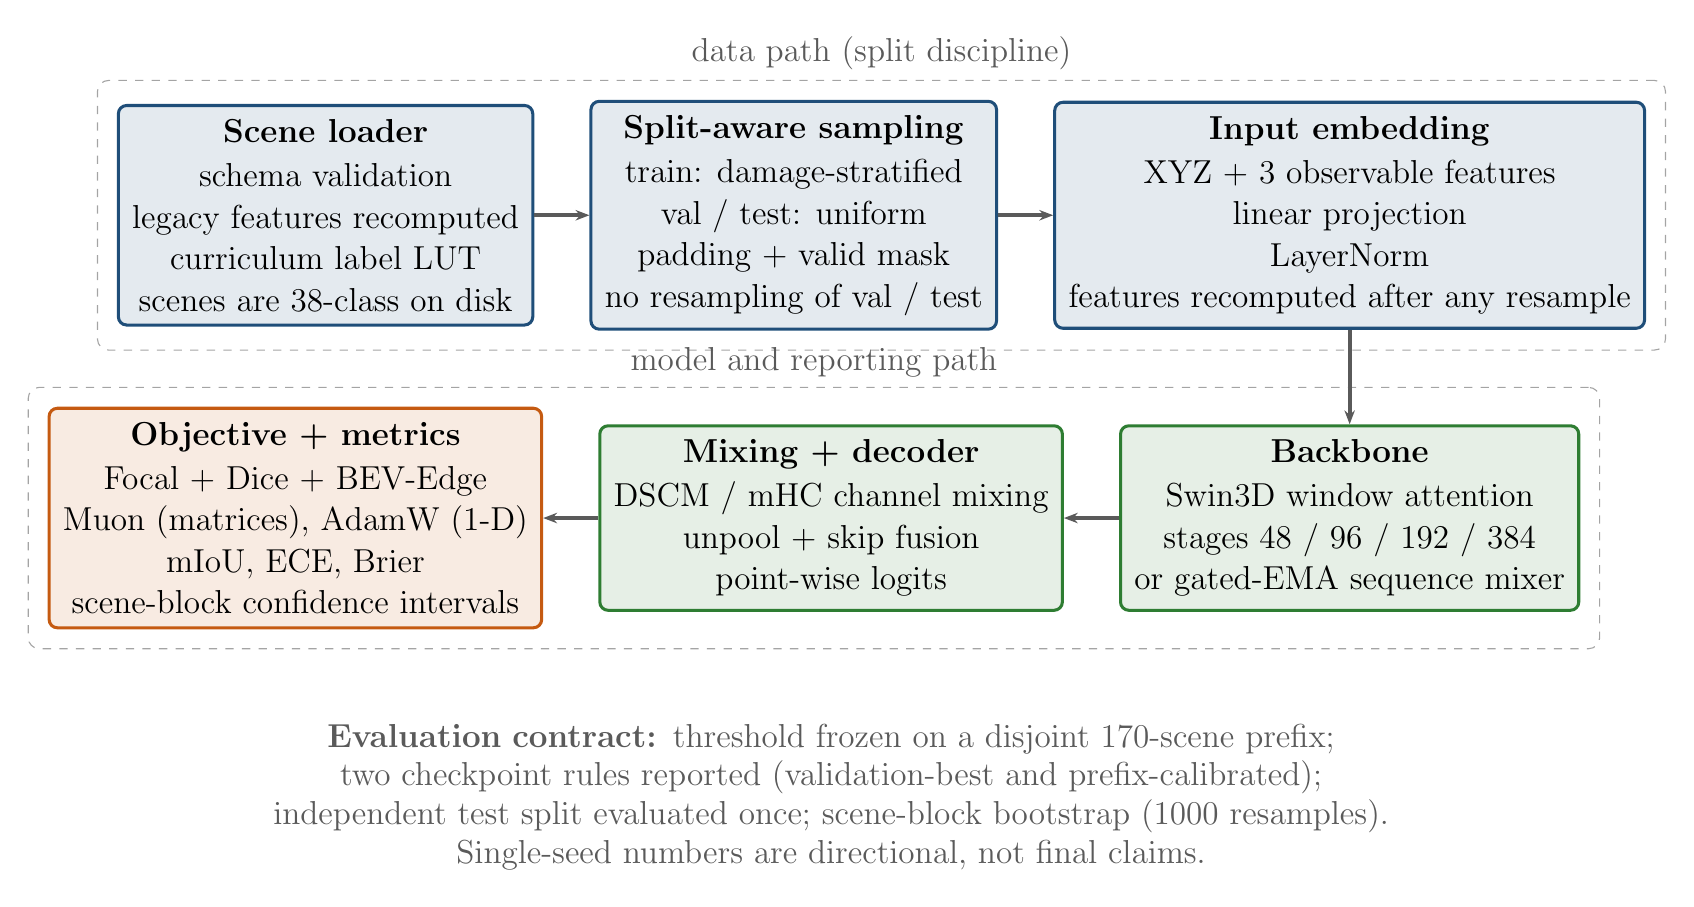
\begin{tikzpicture}[node distance=7mm and 7mm]

% ---------- 第一行：数据路径 ----------
\node[box, fill=cblue!12, draw=cblue] (loader)
  {\textbf{Scene loader}\\[1pt] schema validation\\ legacy features recomputed\\ curriculum label LUT\\ scenes are 38-class on disk};

\node[box, fill=cblue!12, draw=cblue, right=of loader] (sample)
  {\textbf{Split-aware sampling}\\[1pt] train: damage-stratified\\ val / test: uniform\\ padding + valid mask\\ no resampling of val / test};

\node[box, fill=cblue!12, draw=cblue, right=of sample] (embed)
  {\textbf{Input embedding}\\[1pt] XYZ + 3 observable features\\ linear projection\\ LayerNorm\\ features recomputed after any resample};

% ---------- 第二行：模型与报告路径 ----------
\node[box, fill=cgreen!12, draw=cgreen, below=12mm of embed] (backbone)
  {\textbf{Backbone}\\[1pt] Swin3D window attention\\ stages 48 / 96 / 192 / 384\\ or gated-EMA sequence mixer};

\node[box, fill=cgreen!12, draw=cgreen, left=of backbone] (decode)
  {\textbf{Mixing + decoder}\\[1pt] DSCM / mHC channel mixing\\ unpool + skip fusion\\ point-wise logits};

\node[box, fill=camber!12, draw=camber, left=of decode] (loss)
  {\textbf{Objective + metrics}\\[1pt] Focal + Dice + BEV-Edge\\ Muon (matrices), AdamW (1-D)\\ mIoU, ECE, Brier\\ scene-block confidence intervals};

\draw[arr] (loader) -- (sample);
\draw[arr] (sample) -- (embed);
\draw[arr] (embed) -- (backbone);
\draw[arr] (backbone) -- (decode);
\draw[arr] (decode) -- (loss);

\begin{scope}[on background layer]
  \node[grp, fit=(loader)(sample)(embed), label={[lab]above:data path (split discipline)}] {};
  \node[grp, fit=(backbone)(decode)(loss), label={[lab]above:model and reporting path}] {};
\end{scope}

% ---------- 底部契约（置于两行方框之外，避免与虚线框相撞） ----------
\node[lab, below=13mm of decode, text width=200mm]
  {\textbf{Evaluation contract:} threshold frozen on a disjoint 170-scene prefix;\\
   two checkpoint rules reported (validation-best and prefix-calibrated);\\
   independent test split evaluated once; scene-block bootstrap (1000 resamples).\\
   Single-seed numbers are directional, not final claims.};

\end{tikzpicture}
\end{document}
